\chapter{PAC učenie}

V tejto kapitole sa budeme zaoberať otázkou toho, ako závisí chyba
algoritmu od veľkosti trénovacej množiny. Konkrétne sa budeme
zaoberať otázkami ako:
\begin{enumerate}
  \item ``Akú OTeChAlg môžeme očakávať pri danej veľkosti trénovacej množiny $t$?'' \label{pac:q1}
  \item ``Pri danom $t$, s akou pravdepodobnosťou nám algoritmus vráti
    hypotézu, ktorej OTeCh je menšia rovná $\varepsilon$?'' \label{pac:q2}
\end{enumerate}
Na základe odpovedí na tieto dve otázky potom budeme schopní zodpovedať
nasledovné (dalo by sa povedať, že ``inverzné'') otázky:
\begin{enumerate}
  \setcounter{enumi}{2}
  \item ``Akú veľkú trénovaciu množinu máme zvoliť, aby sme dosiahli
    dostatočne malú ($\leq \varepsilon$) OTeChAlg?'' \label{pac:q3}
  \item ``Aké $t$ máme zvoliť, aby sme iba s malou pravdepodobnosťou
    ($\leq \delta$) dostali zlú hypotézu (s OTeCh väčšou ako $\varepsilon$)?'' \label{pac:q4}
\end{enumerate}

Odtiaľ sa odvíja názov \emph{PAC učenie} (z anglického
\emph{probably approximately correct learning}). Presnejšie, PAC učenie
sa zaoberá hlavne otázkami \ref{pac:q2} a \ref{pac:q4}; my sa ale budeme
zaoberať všeobecne tým, ako závisia rôzne metriky (OTeChAlg, ...) od
počtu trénovacích príkladov $t$.

Uvedomme si rozdiel medzi otázkami (\ref{pac:q1}, \ref{pac:q3}) a otázkami
(\ref{pac:q2}, \ref{pac:q4}). V prvom zmienenom sa pýtame na očakávaný
prípad; ak ale chceme dosiahnuť dobrú hypotézu nie v očakávanom prípade,
ale zaručene, vieme to zaručiť iba s určitou pravdepodobnosťou. Vždy sa
totiž môže stať (s malou pravdepodobnosťou), že si vytiahneme
nereprezentatívne trénovacie dáta. Je teda nutné hovoriť aj o
veľkosti tejto záruky, takže hranica $\delta$ je potrebná.




\section{Definície, označenia a predpoklady}

Hypotézu $h$ nazveme \emph{zlou}, ak jej OTeCh je väčšia ako $\varepsilon$.
Inak ju nazveme \emph{dobrou}. Tieto pojmy budeme používať tak, aby bola
hranica $\varepsilon$ vždy jasná z kontextu.

Budeme riešiť hlavne binárne klasifikačné úlohy, v ktorých je cieľom pre
každý vstup $x$ povedať, či spĺňa určitú podmienku ($y = 1$) alebo nespĺňa
($y = 0$). Napríklad môžme chcieť rozlíšiť obrázky $32 \times 32$ ktoré
obsahujú aspoň jednu mačku od tých, ktoré mačky neobsahujú. Príklady,
kde $y = 1$ nazveme \emph{pozitívnymi}; ostatné príklady nazveme
\emph{negatívnymi}. Hypotézy v klasifikačných úlohách budeme nazývať
\emph{klasifikátormi}.

Pripomíname, že chyba klasifikátora $h$ sa počíta ako
$$ \Err(h) = \E_{x, y} \left[ h(x) \neq y \right] = \prob_{x, y} \left( h(x) \neq y \right). $$

Budeme pracovať so štandardným modelom učenia (\ref{ch1:stat_lr_fw})
spolu s predpokladom všemohúceho trénovacieho algoritmu (vždy vráti
hypotézu s najmenšou chybou na trénovacej množine). Okrem toho budeme
predpokladať, že množina hypotéz $H$ je \emph{úplná}: existuje v nej
``úplne správny klasifikátor'', ktorý na každom vstupe dáva
správny výsledok, má teda nulovú testovaciu chybu. Tento klasifikátor
je zrejme najlepšou možnou hypotézou v $H$, mohli by sme ho preto značiť
štandardne $h^\star$. My ho ale budeme značiť $c$ ako ``cieľová hypotéza''.
Treba si ale dať pozor, že správnych hypotéz v $H$ môže byť viac, a to
v prípade, keď niektorým vstupy majú v rozdelení $P$ pravdepodobnosť $0$.
(V takom prípade je $c$ ľubovoľná jedna z týchto hypotéz.)

Uvedomme si, že nech si vytiahneme ľubovoľnú trénovaciu množinu $T$,
vďaka úplnosti množiny $H$ v nej vždy vieme nájsť klasifikátor s nulovou
chybou na trénovacej množine. (Napríklad $h^\star$, môžu tam ale byť
aj ďalšie klasifikátory, s odlišnými výstupmi na vstupoch mimo $T$.) Preto
trénovací algoritmus vždy nájde hypotézu s nulovou trénovacou chybou.
Takýto klasifikátor budeme volať \emph{konzistentný klasifikátor};
názov pochádza od toho, že jeho výstupy sú konzistentné s trénovacími
príkladmi.

Za týchto predpokladov si budeme klásť nasledovnú otázku: ktoré
množiny hypotéz $H$ sa dajú naučiť? Pod ``naučením'' sa rozumie to,
že čím viac trénovacích príkladov algoritmu poskytneme, tým lepšiu
hypotézu $\hat{h}_T$ môžeme očakávať; v limite $t \to \infty$ si
môžeme byť takmer určite istí, že dostaneme veľmi dobrú hypotézu.
Toto sformalizujeme do nasledovnej definície:

\begin{definition}
  Množina hypotéz je \emph{PAC$\star$ naučiteľná}, ak pre ľubovoľné pravdepodobnostné
  rozdelenie $P$ nad $X \times Y$, ľubovoľne malé hranice $\varepsilon > 0$ a $\delta > 0$
  existuje hranica $t_0$ na počet trénovacích príkladov taká, že pre všetky
  počty príkladov $t \geq t_0$ platí: zlú hypotézu (s chybou
  aspoň $\varepsilon$) dostaneme iba s malou pravdepodobnosťou
  (nanajvýš $\delta$).
  $$ \forall P: \forall \varepsilon > 0, \delta > 0: \exists t_0: \forall t \geq t_0: \prob_{T \sim P^t} \left( \Err(\hat{h}_T) \geq \varepsilon \right) \leq \delta $$
\end{definition}

Používame názov PAC$\star$ naučiteľná preto, lebo skutočná (v literatúre
zaužívaná) definícia PAC naučiteľnosti je o čosi komplikovanejšia: berie
väčší ohľad na výpočtové detaily, ktorým sa my chceme zatiaľ vyhnúť.





\section{Konečné množiny hypotéz}

V tejto časti sa zameriame na konečné množiny hypotéz. Uvedieme
niekoľko príkladov takých množín: logické formuly obmedzenej
veľkosti, konečné automaty obmedzenej veľkosti, ... V princípe
všetko, v čom nevystupujú reálne čísla; s tým že uvažujeme iba
malé hypotézy.



\subsection{Konečné množiny sú PAC$\star$ naučiteľné}

\begin{theorem} \label{thm:badhypobound}
  Pomocou počtu trénovacích príkladov $t$ vieme zhora odhadnúť
  pravdepodobnosť, že nám algoritmus vráti zlú hypotézu, nasledovne:
  $$ \prob_T(\Err(\hat{h}_T) \geq \varepsilon) \leq |H| \cdot e^{-\varepsilon t} $$
\end{theorem}
\begin{proof}
  Predstavme si, že na začiatku vidíme $0$ trénovacích príkladov,
  a postupne sa nám odkrývajú. Sledujme jednotlivé hypotézy: vždy,
  keď sa odkryje nejaký príklad, môže sa stať, že je nekonzistentný
  s hypotézou. Každú takúto hypotézu zo súťaže vylúčime. Po odkrytí
  všetkých $t$ trénovacích príkladov zostávajú už len tie hypotézy,
  ktoré sú s príkladmi konzistentné a môžu byť výsledkom algoritmu.
  Ak ani jedna z týchto hypotéz nie je zlá, výsledkom bude dobrá
  hypotéza. Aká je pravdepodobnosť, že aspoň jedna z týchto preživších
  hypotéz je zlá?
  
  Nech $h$ je ľubovoľná zlá hypotéza. Pravdepodobnosť, že je konzistentná
  so všetkými $t$ trénovacími príkladmi, je rovná $(1 - \Err(h))^t$,
  čo vieme odhadnúť nasledovne:
  $$(1 - \Err(h))^t \leq (1 - \varepsilon)^t \leq e^{-\varepsilon t}$$
  
  Zlých hypotéz je nanajvýš toľko, koľko je všetkých hypotéz, teda
  $|H|$. Pravdepodobnosť, že aspoň jedna z nich bude konzistentná
  s príkladmi, je nanajvýš súčet pravdepodobností jednotlivých zlých
  hypotéz:
  $$\prob_T(\text{prežije aspoň jedna zlá hypotéza}) \leq |H| \cdot e^{-\varepsilon t}$$
  Odkiaľ dostávame požadovanú nerovnosť.
\end{proof}

Čo ak nás zaujíma druhá otázka: ``Ako závisí chyba algoritmu od počtu
trénovacích príkladov?'' Pri klasifikačných úlohách je táto otázka úzko
spätá s predošlou otázkou, kde sme sa zaujímali o hranice $\varepsilon$
a $\delta$.

\begin{theorem}
  Platí
  $$ \Err(L) \leq \frac{1}{t} \cdot \left( \ln{|H|} + \ln{t} + 1 \right). $$
\end{theorem}
\begin{proof}
  Ak nám algoritmus vráti dobrú hypotézu, vieme jej OTeCh odhadnúť zhora
  ako $\varepsilon$. Ak nám algoritmus vráti zlú hypotézu, jej OTeCh je
  nanajvýš $1$. Z toho dostávame nasledovný horný odhad na OTeChAlg:
  $$ \Err(L) = \E_T \left[ \Err(\hat{h}_T) \right] \leq \prob_T \left( \Err(\hat{h}_T) < \varepsilon \right) \cdot \varepsilon + \prob_T \left( \Err(\hat{h}_T) \geq \varepsilon \right) \cdot 1 $$
  Pritom sčítance na pravej strane vieme odhadnúť zhora:
  $$ \prob_T \left( \Err(\hat{h}_T) < \varepsilon \right) \leq 1 $$
  a druhý sčítanec vieme odhadnúť pomocou predchádzajúcej vety (\ref{thm:badhypobound}).
  Dostávame tak odhad
  $$ \Err(L) \leq 1 \cdot \varepsilon + |H| \cdot e^{-\varepsilon t}. $$
  My sme si ale mohli zvoliť $\varepsilon$ ľubovoľne. Ak teda chceme
  dostať čo najlepší odhad, nájdeme také $\varepsilon$, pre ktoré je výraz
  na pravej strane čo najmenší: zderivujeme a položíme rovné nule:
  \begin{align}
    1 - |H| \cdot t \cdot e^{-\varepsilon t} &= 0 \\
    \varepsilon &= \frac{1}{t} \cdot \left( \ln{|H|} + \ln{t} \right)
  \end{align}
  Odtiaľ dosadením dostaneme požadovaný odhad na chybu algoritmu.
\end{proof}

Na základe týchto dvoch viet vieme sformulovať postačujúce podmienky
na $t$ také, aby boli hranice $\varepsilon$ a $\delta$ dostatočne malé.

\begin{corollary}
  Ľubovoľná konečná množina hypotéz $H$ je PAC$\star$ naučiteľná: pre
  ľubovoľné rozdelenie $P$, ľubovoľne malé hranice $\varepsilon > 0$
  a $\delta > 0$, pre počet trénovacích príkladov $t$ spĺňajúci
  $$ t \geq \frac{1}{\varepsilon} \cdot \left( \ln{|H|} + \ln{\frac{1}{\delta}} \right) $$
  platí, že dostaneme zlú hypotézu iba s malou pravdepodobnosťou.
\end{corollary}
\begin{proof}
  Podľa vety \ref{thm:badhypobound} platí
  $$ \prob_T \left( \Err(\hat{h}_T) > \varepsilon \right) < |H| \cdot e^{-\varepsilon t}.$$
  Stačí nám teda zvoliť také $t$, aby bol výraz na pravej strane nanajvýš
  $\delta$. Odtiaľ dostaneme postačujúci počet trénovacích
  príkladov $t$.
  \begin{align}
    |H| \cdot e^{-\varepsilon t} &\leq \delta \\
    \ln{|H|} - \varepsilon t &\leq \ln{\delta} \\
    \varepsilon t &\geq \ln{|H|} - \ln{\delta} \\
    t &\geq \frac{1}{\varepsilon} \cdot \left( \ln{|H|} + \ln{\frac{1}{\delta}} \right)
  \end{align}
\end{proof}



\subsection{Problém konjunkcie}

Máme $n$ boolovských premenných. Množinou inštancii $X$ sú všetky
možné ohodnotenia týchto premenných, napríklad pre $n = 3$ je jedným
možným priradením $x_1 = 0$, $x_2 = 1$, $x_3 = 0$. Každé priradenie
si vieme predstaviť ako postupnosť bitov dĺžky $n$. Je zrejmé, že
rôznych priradení je $2^n$.

Množinou hypotéz su všetky formuly tvaru $x_{i_1} \land x_{i_2} \land \ldots \land x_{i_k}$.
Sú to teda konjunkcie premenných, s tým že premenné vo formule nesmú
vystupovať negované. Tieto formuly sú chápané ako funkcie, ktoré
vracajú $1$ vtedy, keď dané ohodnotenie premenných spĺňa túto formulu.
Napríklad $x_1 \land x_3 \land x_4$ vráti $1$ na všetkých vstupoch,
kde $x_1 = 1$, $x_3 = 1$ a $x_4 = 1$ (ostatné premenné môžu mať
ľubovoľnú hodnotu). Rôznych hypotéz je zrejme tiež $2^n$.

\paragraph{Metafora.} Vyššie uvedený popis je možno príliš formálny, 
problém sa dá vysvetliť aj prirodzenejším spôsobom. Predstavme
si, že náš kamarát má batoh, do ktorého dal niektoré z $n$ vecí.
My chceme zistiť, ktoré z týchto vecí v batohu sú a ktoré v ňom
nie sú. Množina inštancii sú teda jednotlivé veci, a hypotézy sú
všetky možné obsahy batoha. Čo ale zodpovedá trénovacím príkladom?
Predstavme si, že sa môžeme spýtať niekoľko otázok tvaru: ``Obsahuje
batoh iba týchto $k$ vecí?'' (t.j. nič iné nesmie obsahovať) a kamarát
nám na každú otázku odpovie áno/nie. Potom trénovacie príklady
zodpovedajú práve takýmto otázkam, spolu s odpoveďami na ne.

Zavedieme prirodzenú notáciu pre túto metaforu: namiesto $h(x) = 1$
budeme písať $h \subseteq x$, a namiesto $h(x) = 0$ píšeme $h \not\subseteq x$.

\paragraph{Všemohúci trénovací algoritmus.} Uvidíme, že konzistentnosť
s trénovacími príkladmi je realistická požiadavka: ukážeme, ako sa
dá na základe trénovacích príkladov zostrojiť nejaký konzistentný
klasifikátor.

\begin{theorem}
  Nech hypotéza $\hat{h}_T$ obsahuje všetky tie veci, ktoré sa vyskytujú
  v každom pozitívnom trénovacom príklade. Potom $\hat{h}$ je
  konzistentná so všetkými trénovacími príkladmi.
\end{theorem}
\begin{proof}
  Ak $(x, y)$ je pozitívny príklad, v batohu môže byť iba nejaká podmnožina
  vecí z $x$. Keď túto úvahu zopakujeme pre všetky pozitívne príklady,
  dostaneme niekoľko množín ``povolených vecí''. Skutočný obsah batoha
  musí byť podmnožinou všetkých z nich, teda je podmnožinou ich prieniku.
  Toto zároveň zachytáva všetku informáciu zo všetkých pozitívnych príkladov,
  teda ľubovoľná hypotéza, ktorá je podmnožinou tohto prieniku,
  je konzistentná s pozitívnymi príkladmi.
  
  Čo ale s negatívnymi príkladmi? Ak by sme zobrali príliš malú
  množinu vecí ako hypotézu, mohol by nastať problém s negatívnymi
  príkladmi. (Napríklad ak máme príklady $(0110, 0)$ a $(1100, 1)$,
  nemôžeme ako hypotézu zvoliť $0100$ ani $0000$, lebo by to bolo
  v rozpore s prvým príkladom.)
  
  Ak ale zoberieme celý prienik ako našu hypotézu $\hat{h}_T$, nemôže
  sa to stať. Totiž, skutočný obsah batoha je podmnožinou oného
  prieniku, a teda ak $\hat{h}_T \subseteq x$, tak nutne aj
  $c \subseteq x$. Obmenou tejto implikácie dostaneme, že ak
  $c \not\subseteq x$, tak aj $\hat{h}_T \not\subseteq x$, takže
  naša hypotéza dáva na negatívnych príkladoch rovnaké výsledky.
\end{proof}

Uvedieme teraz niektoré výsledky z predchádzajúcej časti tak, ako platia
pre problém konjunkcie.

\begin{theorem}
  Pre problém konjunkcie platí
  $$ \Err(L) \leq \frac{1}{t} \cdot \left( n \ln{2} + \ln{t} + 1 \right) = O\left( \frac{n + \ln{t}}{t} \right). $$
\end{theorem}
\begin{theorem} \label{cor:mconj_de}
  Pre problém konjunkcie platí, že aby sme zlú hypotézu (s chybou aspoň
  $\varepsilon$) dostali iba s malou pravdepodobnosťou (nanajvýš $\delta$),
  stačí zvoliť veľkosť trénovacej množiny nasledovne:
  $$ t \geq \frac{1}{\varepsilon} \cdot \left( n \ln{2} + \ln{\frac{1}{\delta}} \right) = \Omega\left( \frac{n + \ln{\frac{1}{\delta}}}{\varepsilon} \right) $$
\end{theorem}

\paragraph{Dolné odhady.} Tieto odhady sú relatívne tesné. Ako veľmi ich
vieme zlepšiť? Vieme dostať aj nejaké dolné odhady, t.j. tvrdenia hovoriace,
že ak sa chceme nejakú množinu hypotéz naučiť, potrebujeme aspoň toľkoto
trénovacích príkladov?

Netriviálny dolný odhad na všetky prípady sa nedá dostať, nakoľko
pravdepodobnostné rozdelenie $P$ môže byť degenerované a ``uľahčiť
algoritmu robotu''. (Napríklad keď $P$ priradí všetkých $100\%$
jednej dvojici $(x, y)$.) Prirodzenejšie je teda hľadať nejaké
jedno ťažké rozdelenie $P$. Toto rozdelenie ale môže závisieť od
konkrétneho trénovacieho algoritmu; nestačí len predpokladať, že
algoritmus je všemohúci, nakoľko možných výsledných hypotéz môže
byť viacero a ťažkosť rozdelenia $P$ závisí od toho, ako sa hypotéze
darí mimo trénovacích príkladov.

Budeme teda hľadať tvrdenia tvaru: pre každý algoritmus $L$ existuje
rozdelenie $P$, na ktorom potrebuje $L$ aspoň nejaké množstvo trénovacích
príkladov, aby sa mu dobre darilo.

Dokazovať to v takomto tvare sa ale ukazuje byť ťažké. Problém je v tom,
že nájsť konkrétne ťažké rozdelenie $P$ môže byť ťažké. V matematike nie vždy
vieme ľahko nájsť konkrétny príklad s nejakou vlastnosťou; možno ale
vieme ľahko dokázať, že taký objekt musí existovať. Tak tomu bude aj teraz;
v dôkaze budeme využívať nasledovnú všeobecnú metavetu:

\begin{theorem}
  Ak chceme dokázať, že existuje objekt $o$ spĺňajúci $f(o) \geq l$,
  kde $f$ reprezentuje nejakú vlastnosť objektu $o$ a hodnota $l$
  je nejaká ľubovoľná hranica, stačí dokázať, že pre $o$ náhodne
  vybrané z nejakého rozdelenia $O$ platí
  $$ \E_{o \sim O} \left[ f(o) \right] \geq l. $$
\end{theorem}
\begin{proof}
  Ak je hodnota $f(o)$ v priemere aspoň $l$, tak aspoň v jednom konkrétnom
  prípade (t.j. pre jedno konkrétne $o$) musí byť tiež väčšia rovná $l$.
  Formálne zapísaná obmena tejto implikácie:
  $$ (\forall o \in O: f(o) < l) \implies \E_{o \sim O} \left[ f(o) \right] < l. $$
\end{proof}

V našom prípade namiesto hľadania jedného konkrétneho ťažkého
rozdelenia $P$ ho zvolíme náhodne. Potom ukážeme, že OTeChAlg
bude vysoká (pričom stredná hodnota sa berie aj cez náhodné voľby
rozdelenia $P$).

\begin{theorem} \label{thm:mconj_lb}
  Pre problém konjunkcie platí, že pre ľubovoľný algoritmus $L$ existuje
  rozdelenie $P$ také, že pre $t \geq n - 1$ platí pre OTeChAlg platí
  nasledovný dolný odhad:
  $$ \Err(L) \geq \frac{1}{2e} \cdot \frac{n-1}{t+1} = \Omega \left( \frac{n}{t} \right)$$
  Pre $t < n - 1$ platí iný dolný odhad:
  $$ \Err(L) \geq \frac{1}{2e} = \Omega \left( 1 \right). $$
\end{theorem}
\begin{proof}
  Predstavme si, že v rozdelení $P$ vystupujú (t.j. majú nenulovú
  pravdepodobnosť) iba tie vstupy, ktoré obsahujú presne $n - 1$
  vecí, teda práve jedna vec v množine nie je. Označme tieto vstupy
  $x^{(1)}, \ldots, x^{(n)}$ podľa toho, ktorá vec chýba.
  
  Ľubovoľná hypotéza $h$ vráti na vstupe $x^{(i)}$ hodnotu $1$ práve
  vtedy, keď vec $i$ v hypotéze nie je; hodnotu $0$ vráti vtedy, keď tam
  vec $i$ je. Tieto vstupy teda zodpovedajú otázkam tvaru:
  ``Je pravda, že vec $v$ nie je v batohu?''
  
  Takže každý trénovací príklad nám dáva informáciu iba o prítomnosti
  jednej veci. Počas testovania teda vieme správnu odpoveď iba na
  tých vstupoch, ktoré sme dostali ako trénovacie príklady. Na ostatných
  môžeme vo všeobecnosti iba hádať, či v batohu príslušná vec je alebo
  nie je.
  
  Takže na vstupoch, ktoré sú v trénovacej množine, budeme mať chybu $0$.
  Ak bol obsah batoha (t.j. výstupy $y$) zvolený rovnomerne náhodne
  spomedzi všetkých $2^n$ možností, tak na ostatných vstupoch budeme
  mať očakávanú chybu $\frac{1}{2}$.
  
  Označme si pravdepodobnosti pridelené jednotlivým vstupom $p_1, \ldots, p_n$.
  OTeChAlg vieme zmerať tak, že si náhodne vytiahneme trénovacie príklady
  a náhodne vytiahneme testovací príklad. Potom na trénovacích príkladoch
  natrénujeme hypotézu $\hat{h}_T$, zmeriame jej chybu na testovacom príklade,
  a spravíme strednú hodnotu tohto procesu. Aká je šanca, že pri trénovaní
  vstup $x^{(i)}$ nedostaneme a potom si ho pri testovaní vytiahneme?
  $$p_i \cdot (1 - p_i)^t$$
  
  Celková pravdepodobnosť, že si pri testovaní vytiahneme vstup
  mimo trénovacej množiny, je potom súčtom týchto pravdepodobností
  cez všetky vstupy $x^{(i)}$:
  $$\sum_{i=1}^n p_i \cdot (1 - p_i)^t$$
  
  Tieto prípady prispievajú do chyby $1/2$, ostatné prípady prispievajú $0$.
  Dostávame tak nasledovný dolný odhad na chybu algoritmu:
  $$ \Err(L) \geq \frac{1}{2} \cdot \left( \sum_{i=1}^n p_i \cdot (1 - p_i)^t \right) $$
  
  Ako zvoliť $p_1, \ldots, p_n$ tak, aby sme dostali dobrý dolný
  odhad? Skúsme zvoliť $p_i$ také, pre ktoré nadobúda výraz
  $p_i \cdot (1 - p_i)^t$ maximum. Zderivovaním a položením
  rovné $0$ dostaneme
  $$p_i = \frac{1}{t+1}.$$
  
  Pokiaľ $t \neq n - 1$, nemôžeme zvoliť všetky pravdepodobnosti
  takéto: pre $t > n - 1$ by bol súčet pravdepodobností primalý
  a pre $t < n - 1$ priveľký. Rozoberme tieto prípady osobitne.
  
  \paragraph{Prvý prípad ($t \geq n - 1$).} Všetkým vstupom okrem jedného
  priradíme pravdepodobnosť $1/(t+1)$; posledný vstup dostane všetkú zvyšnú
  pravdepodobnosť.
  $$ p_1 = p_2 = \ldots = p_{n-1} = \frac{1}{t+1},\ p_n = 1 - \frac{n-1}{t+1}$$
  Dosadíme a dostaneme tak odhad
  $$ \Err(L) \geq \frac{1}{2} \cdot \left( (n - 1) \cdot \frac{1}{t+1} \cdot \left( 1 - \frac{1}{t+1} \right)^t + \frac{n-1}{t+1} \cdot \left( 1 - \frac{n-1}{t+1} \right)^t \right). $$
  Druhý sčítanec zdola odhadneme ako $0$ a ďalej použijeme odhad
  $$ \left( 1 - \frac{1}{t+1} \right)^t \geq \frac{1}{e}, $$
  ktorý platí pre všetky prirodzené $t$. Dostaneme tak nerovnosť
  $$ \Err(L) \geq \frac{1}{2e} \cdot \frac{n-1}{t+1}. $$
  
  \paragraph{Druhý prípad ($t < n - 1$).} Prvým $t+1$ vstupom priradíme
  pravdepodobnosť $1/(t+1)$, ostatné vstupy dostanú pravdepodobnosť $0$.
  Dostaneme tak odhad
  \begin{align}
    \Err(L) &\geq \frac{1}{2} \cdot (t + 1) \cdot \frac{1}{t+1} \cdot \left( 1 - \frac{1}{t+1} \right)^t \\
    \Err(L) &\geq \frac{1}{2e}
  \end{align}
\end{proof}

\begin{comment}
Dolný odhad zodpovedajúci dôsledku \ref{cor:mconj_de} uvedieme bez dôkazu.

\begin{theorem}
  Pre ľubovoľný trénovací algoritmus existuje pravdepodobnostné rozdelenie
  $P$ a cieľová hypotéza $f \in H$, ktoré vynútia, že algoritmus bude
  potrebovať aspoň
  $$ t = \Omega \left( \frac{1}{\varepsilon} \cdot \left( n + \ln{\frac{1}{\delta}} \right) \right), $$
  aby platilo
  $$ \prob(\err(\hat{h}) > \varepsilon) \leq \delta.$$
\end{theorem}

\TODO{dôkaz}
\end{comment}




\section{Nekonečné množiny hypotéz}

Vyššie uvedené postupy pre konečné množiny hypotéz zlyhajú, ak
$|H| = \infty$. Aj pre nekonečné množiny hypotéz je ale možné
odvodiť horné odhady. Tie sa už nebudú odvíjať od veľkosti množiny $H$,
ale od nejakej jej miery zložitosti. Touto mierou zložitosti bude tzv.
\emph{Vapnik-Chervonenkisova dimenzia}. Najprv sa ale pozrieme
na jednoduchý príklad.




\subsection{Obdĺžniková hra}

Množinou inštancii sú všetky body roviny a množinou hypotéz sú všetky
obdĺžniky, ktorých strany sú rovnobežné so súradnicovými osami. Obdĺžnik
chápeme ako funkciu, ktorá vracia $1$ pre tie body, ktoré sú vo vnútri
obdĺžnika (vrátane jeho okrajov).

Pre jednoduchosť argumentu použijeme konkrétny trénovací algoritmus.
Dôkaz by sa dal zovšeobecniť na prípad, kedy jediné, čo o algoritme
predpokladáme je to, že je všemohúci. S nasledovným konkrétnym algoritmom
ale bude analýza jednoduchšia.

\paragraph{Všemohúci trénovací algoritmus.} Z trénovacích príkladov 
vezmeme tie pozitívne, a ako náš obdĺžnik $\hat{h}_T$ zvolíme najmenší
osovorovnobežný obdĺžnik obsahujúci body z týchto príkladov (tzv.
\emph{bounding box}). Túto konštrukciu ilustrujeme na obrázku \ref{rectgame:hath}.

Takýto obdĺžnik zrejme obsahuje všetky pozitívne
trénovacie príklady, je teda s nimi konzistentný. Pretože je to najmenší
taký obdĺžnik, musí byť celý vo vnútri cieľového obdĺžnika. Nemôže sa teda
stať, že by nejaký bod nepatril do $c$ ale patril do nášho obdĺžnika; je
teda konzistentný aj s negatívnymi trénovacími príkladmi.

\begin{figure}
  \centering
  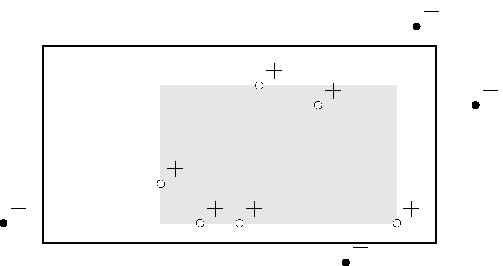
\includegraphics[scale=1]{obrazky/rectgame1.pdf}
  \caption{
    Obdĺžniková hra: najmenší obdĺžnik konzistentný s príkladmi
    v porovnaní s cieľovým obdĺžnikom.
  }
  \label{rectgame:hath}
\end{figure}

\begin{theorem}
  Obdĺžniková hra je PAC$\star$ naučiteľná: pre ľubovoľné rozdelenie $P$,
  ľubovoľne malé hranice $\varepsilon > 0$ a $\delta > 0$, ak pre počet
  pozitívnych trénovacích príkladov $t^+$ platí
  $$ t^+ \geq \frac{4}{\varepsilon} \cdot \ln{\frac{4}{\delta}}, $$
  tak nám algoritmus vráti zlú hypotézu (s OTeCh aspoň $\varepsilon$)
  iba s malou pravdepodobnosťou (nanajvýš $\delta$).
\end{theorem}

Všimnime si, že v našom tvrdení vystupuje $t^+$ namiesto $t$. Ak
rozdelenie $P$ vráti pozitívny príklad s nenulovou pravdepodobnosťou,
nie je to problém: s veľkým počtom trénovacích príkladov $t$ potom vieme
dosiahnuť aj veľký počet pozitívnych trénovacích príkladov $t^+$.

Čo ak rozdelenie $P$ pozostáva iba z negatívnych príkladov? V takom
prípade náš algoritmus nepotrebuje žiaden príklad, hneď dosiahne OTeCh
$100\%$. Vždy totiž vráti degenerovaný obdĺžnik, ktorý neobsahuje žiadne
body (ani len na okraji).

V dôkaze budeme riešiť už len prvý prípad.

\begin{proof}
  Pod \emph{váhou} množiny budeme rozumieť pravdepodobnosť, že náhodný
  bod z rozdelenia $P$ padne do tejto množiny.

  Zle klasifikované body roviny sú tie, ktoré sú vo vnútri cieľového obdĺžnika
  $c$ ale nie sú vo vnútri nášho obdĺžnika $\hat{h}_T$. Každý z týchto zlých
  bodov padne do aspoň jedného z pásov na okraji $c$, ako je vyobrazené
  na obrázku \ref{rectgame:strips}.

  Zlá hypotéza je taká, v ktorej je celková váha zlých bodov aspoň $\varepsilon$.
  Kedže každý zlý bod padne do aspoň jedného z pásov, aspoň jeden z týchto pásov
  musí mať váhu aspoň $\varepsilon/4$. To ale znamená, že ak žiaden z pásov
  nebude mať takúto veľkú váhu, naša hypotéza bude zaručene dobrá. Inými
  slovami, pravdepodobnosť zlej hypotézy je zhora ohraničená pravdepodobnosťou,
  že aspoň jeden z pásov má váhu aspoň $\varepsilon/4$.
  
  Pozrime sa na ľubovoľný jeden konkrétny pás, BUNV ten ľavý. Aká je
  pravdepodobnosť, že váha tohto pásu je aspoň $\varepsilon/4$? Aby sa
  toto stalo, museli by všetky body z trénovacích príkladov padnúť
  ďaleko od ľavého okraja. Ako presne ďaleko?
  
  Predstavme si súvislý úsek bodov od ľavého okraja, ktorého váha je
  presne $\varepsilon/4$. Bod je dostatočne ďaleko, ak nepadne do tohto
  úseku; ilustrujeme na obrázku \ref{rectgame:eps_strip}. Pravdepodobnosť,
  že náhodný príklad padne takto ďaleko, je $1 - \varepsilon/4$; pravdepodobnosť,
  že každý z $t$ náhodne vybraných trénovacích príkladov padol takto ďaleko,
  je $(1 - \varepsilon/4)^t$.
  
  S touto predstavou je ale drobný technický problém: nie pre každé
  rozdelenie $P$ platí, že vieme nájsť úsek s váhou presne $\varepsilon/4$.
  Napríklad si predstavme rozdelenie, v ktorom s pravdepodobnosťou $50\%$
  dostaneme bod v strede obdĺžnika, a inak si vyberieme rovnomerne náhodne
  bod v pravej polovici. Najmenší ľavý súvislý úsek s kladnou váhou bude mať
  hneď váhu $50\%$.
  
  Musíme teda postupovať inak. Uvedomme si, že bod $x$ je dostatočne ďaleko vtedy, keď váha bodov naľavo
  od $x$ je aspoň $\varepsilon/4$. To ale znamená, že vieme vyznačiť súvislý
  úsek bodov pri ľavom okraji, ktorý má váhu aspoň $\varepsilon/4$ a ktorý
  je celý naľavo od všetkých takýchto dostatočne vzdialených bodov $x$.
  Z toho vyplýva, že váha všetkých dostatočne vzdialených bodov môže
  byť nanajvýš $1 - \varepsilon/4$. Pravdepodobnosť, že náhodný príklad
  padne takto ďaleko, je preto nanajvýš $1 - \varepsilon/4$; pravdepodobnosť,
  že každý z $t$ náhodne vybraných trénovacích príkladov padol takto ďaleko,
  je nanajvýš $(1 - \varepsilon/4)^t$. To ďalej zhora odhadneme ako $e^{-t \cdot \varepsilon/4}$.
  
  Tento odhad spravíme pre každý z okrajových pásov. Dostaneme tak
  odhad na pravdepodobnosť zlej hypotézy:
  $$ \prob_T \left( \Err(\hat{h}_T) \geq \varepsilon \right) \leq 4 \cdot e^{-\frac{t \varepsilon}{4}} $$

  Ak chceme dostať zlú hypotézu iba s malou pravdepodobnosťou (nanajvýš $\delta$),
  stačí zvoliť také $t$, že pravá strana je nanajvýš $\delta$. Odtiaľ dostaneme
  odhad na postačujúci počet trénovacích príkladov:
  \begin{align}
    4 \cdot e^{-\frac{t \varepsilon}{4}} &\leq \delta \\
    -\frac{t \varepsilon}{4} &\leq \ln \left( \frac{\delta}{4} \right) \\
    t &\geq \frac{4}{\varepsilon} \cdot \ln \left( \frac{4}{\delta} \right)
  \end{align}
  
  \begin{figure}
    \begin{subfigure}[t]{0.49\linewidth}
      \centering
      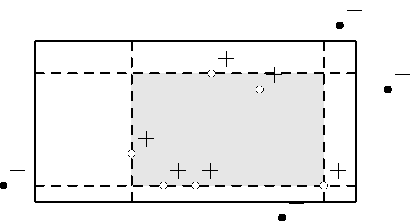
\includegraphics[scale=1]{obrazky/rectgame2.pdf}
      \caption{Krajné pásiky.}
      \label{rectgame:strips}
    \end{subfigure}
    ~
    \begin{subfigure}[t]{0.49\linewidth}
      \centering
      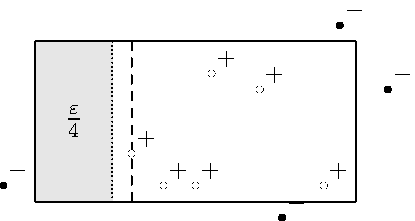
\includegraphics[scale=1]{obrazky/rectgame3.pdf}
      \caption{Sivou farbou je vyznačený súvislý úsek bodov s váhou
        presne $\varepsilon/4$.}
      \label{rectgame:eps_strip}
    \end{subfigure}
    \caption{Obdĺžniková hra.}
  \end{figure}
\end{proof}




\subsection{Vapnik-Chervonenkisova dimenzia}

Vapnik-Chervonenkisova dimenzia (alebo skrátene VC dimenzia) je miera
zložitosti množiny hypotéz, pomocou ktorej sme schopní tvoriť tvrdenia
v štýle PAC učenia. Na jej definíciu budeme potrebovať niekoľko pomocných
pojmov.

\begin{definition}
  Majme konečnú podmnožinu vstupov $S \subseteq X$. Hovoríme, že množina
  hypotéz $H$ \emph{rozbíja} množinu $S$, ak platí: nech označíme vstupy
  v $S$ ako pozitívne alebo negatívne akokoľvek, v množine $H$ existuje
  hypotéza konzistentná s týmto označením.
\end{definition}

Intuitívne, množina $S$ je rozbitá hypotézami $H$, ak nie je pre
hypotézy v $H$ príliš náročné modelovať príklady v $S$: sú schopné
ich modelovať akokoľvek.

\begin{definition}
  Vapnik-Chervonenkisova dimenzia množiny hypotéz $H$, označovaná
  $VCD(H)$, je veľkosť najväčšej množiny $S \subseteq X$, ktorá
  sa dá rozbiť hypotézami v $H$. Ak sa dá rozbiť ľubovoľne veľká
  množina $S$, definujeme $VCD(H) = \infty$.
\end{definition}

Teda na to, aby sme ukázali dolný odhad $VCD(H) \geq d$, stačí nám
nájsť jednu množinu $S$ veľkosti $d$, ktorá sa dá rozbiť. Aby sme ale
ukázali horný odhad $VCD(H) \leq d$, musíme ukázať, že žiadna množina
veľkosti $d + 1$ sa nedá rozbiť: teda že existuje také označenie vstupov,
pre ktoré neexistuje v $H$ konzistentný klasifikátor. Z tohto dôvodu je
obvykle ťažšie dokázať horný odhad na VC dimenziu, ako dolný odhad.

\begin{lemma}
  Majme dve množiny hypotéz $H$ a $H'$ nad tou istou množinou vstupov $x$.
  Ak platí $H \supseteq H'$, tak potom platí $VCD(H) \succeq VCD(H')$ (kde
  $\succeq$ je relácia $\geq$ prirodzene rozšírená na $\N \cup \{ \infty \}$).
\end{lemma}
\begin{proof}
  Ak sa množina $S$ dá rozbiť pomocou $H'$, potom, pretože každá hypotéza
  v $H'$ je aj v $H$, dá sa táto množina rozbiť aj pomocou $H$ (rovnakým
  spôsobom).
\end{proof}

Než uvedieme vety hovoriace o PAC naučiteľnosti, uvedieme príklady
niektorých nekonečných množín hypotéz, a neformálne zdôvodníme ich
VC dimenzie. Väčšinou budú geometrického charakteru (čo je prirodzené,
ak máme mať nekonečnú množinu hypotéz).

\paragraph{Intervaly na reálnych číslach.} Nie je ťažké vidieť, že
ľubovoľná dvojica bodov sa dá rozbiť. Na druhej strane, ak máme tri
body, tak ich vieme označiť ako na obrázku \ref{vc:interval}, čo nie
je konzistentné so žiadnym intervalom. Takže VC dimenzia je $2$.

\begin{figure}
  \centering
  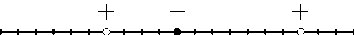
\includegraphics[scale=1]{obrazky/interval.pdf}
  \caption{Žiaden interval nevytvorí takéto označenie bodov.}
  \label{vc:interval}
\end{figure}

\paragraph{Polroviny v rovine.} Každá trojica bodov tvoriacich
nedegenerovaný trojuholník sa dá rozbiť, ako je ilustrované na
obrázku \ref{vc:halfplane}. Na druhej strane, žiadna štvorica bodov
sa rozbiť nedá: ak tvoria konvexný štvoruholník, tak jednu protiľahlú 
dvojicu označíme kladne a druhú záporne. Ak tvoria nekonvexný 
štvoruholník, jeden z bodov je vo vnútri trojuholníka tvoreného 
ostatnými tromi: tento bod označíme kladne a ostatné body záporne.
Takže VC dimenzia je $3$.

\begin{figure}
  \centering
  \begin{subfigure}[b]{0.3\linewidth}
    \centering
    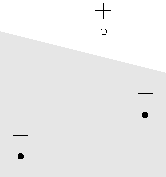
\includegraphics[scale=1]{obrazky/halfplane1.pdf}
    \caption{}
  \end{subfigure}
  ~
  \begin{subfigure}[b]{0.3\linewidth}
    \centering
    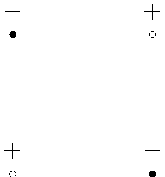
\includegraphics[scale=1]{obrazky/halfplane2.pdf}
    \caption{}
  \end{subfigure}
  ~
  \begin{subfigure}[b]{0.3\linewidth}
    \centering
    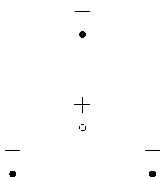
\includegraphics[scale=1]{obrazky/halfplane3.pdf}
    \caption{}
  \end{subfigure}
  \caption{Polroviny v rovine: v situácii (a) vieme nájsť deliacu priamku, v (b) a (c) nie.}
  \label{vc:halfplane}
\end{figure}

\paragraph{Osovorovnobežné obdĺžniky.} Štvorica bodov, ktorá sa dá
rozbiť, je ilustrovaná na obrázku \ref{vc:rect}, nie každá štvorica
bodov sa ale dá rozbiť. Na druhej strane, žiadna pätica bodov sa nedá
rozbiť. Rozoberieme dva prípady: ak je aspoň jeden z bodov vo vnútri 
bounding boxu (nie na okraji), tak ho označíme záporne a všetky body na 
okraji kladne. Ak sú všetky body na obvode bounding boxu, na jednej 
strane toho obdĺžnika musia ležať aspoň dva body. Jeden z nich označíme 
kladne a druhý záporne. Takže VC dimenzia je $4$.

\begin{figure}
  \centering
  \begin{subfigure}[b]{0.23\linewidth}
    \centering
    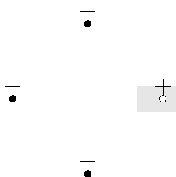
\includegraphics[scale=1]{obrazky/vc_rect1.pdf}
    \caption{}
  \end{subfigure}
  ~
  \centering
  \begin{subfigure}[b]{0.23\linewidth}
    \centering
    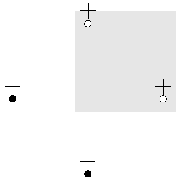
\includegraphics[scale=1]{obrazky/vc_rect2.pdf}
    \caption{}
  \end{subfigure}
  ~
  \centering
  \begin{subfigure}[b]{0.23\linewidth}
    \centering
    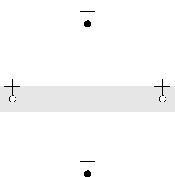
\includegraphics[scale=1]{obrazky/vc_rect3.pdf}
    \caption{}
  \end{subfigure}
  ~
  \centering
  \begin{subfigure}[b]{0.23\linewidth}
    \centering
    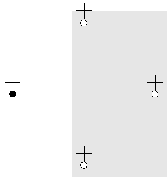
\includegraphics[scale=1]{obrazky/vc_rect4.pdf}
    \caption{}
  \end{subfigure}
  \caption{Osovorovnobežné obdĺžniky: štvorica bodov, ktorá sa dá rozbiť.
    Jednotlivé obrázky zobrazujú všetky netriviálne označenia bodov a
    príslušné konzistentné klasifikátory.}
  \label{vc:rect}
\end{figure}

\medskip

Nakoniec hlavný výsledok, kvôli ktorému je VC dimenzia zaujímavá.

\begin{theorem}[Blumer et. al., 1989 \cite{blumer1989learnability}]
  Nech $C$ je ľubovoľná množina konceptov. Nech $H$ je množina hypotéz
  s VC dimenziou rovnou $d$. Nech $L$ je ľubovoľný algoritmus, ktorý
  pre ľubovoľnú sadu $t$ trénovacích príkladov vráti hypotézu $\hat{h}$
  konzistentnú s príkladmi. Potom $L$ je PAC trénovací algoritmus pre
  množinu konceptov $C$ s použitím hypotéz v $H$, pokiaľ je $t$
  dostatočne veľké:
  $$ t \geq c_0 \left( \frac{1}{\varepsilon} \ln{\frac{1}{\delta}} + \frac{d}{\varepsilon} \ln{\frac{1}{\varepsilon}} \right) $$
  pre nejakú konštantu $c_0 > 0$.
\end{theorem}

\TODO{dôkaz}

\begin{theorem}[Haussler et. al., 1994 \cite{haussler1994predicting}]
  Ak VC dimenzia je $d$, tak ľubovoľný trénovací algoritmus, ktorý vždy
  vracia hypotézy konzistentné s trénovacími príkladmi, má chybu nanajvýš
  $$ \E \left[ \err(\hat{h}) \right] = O\left( \frac{d}{t} \ln{\frac{t}{d}} \right). $$
\end{theorem}

\TODO{dôkaz}

Čo ale v prípade, že neexistuje konzistentný klasifikátor? Taká situácia
nastane, keď buď cieľový koncept nie je v množine hypotéz, alebo keď v
probléme vystupuje šum. Ukazuje sa, že aj v takom prípade sa dá
odhadnúť chyba hypotézy.

\begin{theorem}[Vapnik \& Chervonenkis, 1971 \cite{chervonenkis1971theory}]
  Nech $h^\star$ je hypotéza v $H$ s najmenšou (testovacou) chybou a
  nech $\hat{h}$ je hypotéza v $H$ s najmenšou trénovacou chybou. Ak
  $VCD(H) = d$, tak pre počet trénovacích príkladov
  $$ t \geq c_0 \left( \frac{1}{\varepsilon} \ln{\frac{1}{\delta}} + \frac{d}{\varepsilon} \ln{\frac{1}{\varepsilon}} \right), $$
  kde $c_0$ je nejaká konštanta, platí, že s veľkou pravdepodobnosťou
  je chyba hypotézy $\hat{h}$ dostatočne malá (berúc v úvahu najmenšiu
  dosiahnuteľnú chybu):
  $$ \prob( \err(\hat{h}) > \err(h^\star) + \varepsilon ) \leq \delta. $$
\end{theorem}

\TODO{dôkaz}
